% Options for packages loaded elsewhere
\PassOptionsToPackage{unicode}{hyperref}
\PassOptionsToPackage{hyphens}{url}
%
\documentclass[
]{article}
\usepackage{amsmath,amssymb}
\usepackage{lmodern}
\usepackage{ifxetex,ifluatex}
\ifnum 0\ifxetex 1\fi\ifluatex 1\fi=0 % if pdftex
  \usepackage[T1]{fontenc}
  \usepackage[utf8]{inputenc}
  \usepackage{textcomp} % provide euro and other symbols
\else % if luatex or xetex
  \usepackage{unicode-math}
  \defaultfontfeatures{Scale=MatchLowercase}
  \defaultfontfeatures[\rmfamily]{Ligatures=TeX,Scale=1}
\fi
% Use upquote if available, for straight quotes in verbatim environments
\IfFileExists{upquote.sty}{\usepackage{upquote}}{}
\IfFileExists{microtype.sty}{% use microtype if available
  \usepackage[]{microtype}
  \UseMicrotypeSet[protrusion]{basicmath} % disable protrusion for tt fonts
}{}
\makeatletter
\@ifundefined{KOMAClassName}{% if non-KOMA class
  \IfFileExists{parskip.sty}{%
    \usepackage{parskip}
  }{% else
    \setlength{\parindent}{0pt}
    \setlength{\parskip}{6pt plus 2pt minus 1pt}}
}{% if KOMA class
  \KOMAoptions{parskip=half}}
\makeatother
\usepackage{xcolor}
\IfFileExists{xurl.sty}{\usepackage{xurl}}{} % add URL line breaks if available
\IfFileExists{bookmark.sty}{\usepackage{bookmark}}{\usepackage{hyperref}}
\hypersetup{
  hidelinks,
  pdfcreator={LaTeX via pandoc}}
\urlstyle{same} % disable monospaced font for URLs
\usepackage[margin=1in]{geometry}
\usepackage{graphicx}
\makeatletter
\def\maxwidth{\ifdim\Gin@nat@width>\linewidth\linewidth\else\Gin@nat@width\fi}
\def\maxheight{\ifdim\Gin@nat@height>\textheight\textheight\else\Gin@nat@height\fi}
\makeatother
% Scale images if necessary, so that they will not overflow the page
% margins by default, and it is still possible to overwrite the defaults
% using explicit options in \includegraphics[width, height, ...]{}
\setkeys{Gin}{width=\maxwidth,height=\maxheight,keepaspectratio}
% Set default figure placement to htbp
\makeatletter
\def\fps@figure{htbp}
\makeatother
\setlength{\emergencystretch}{3em} % prevent overfull lines
\providecommand{\tightlist}{%
  \setlength{\itemsep}{0pt}\setlength{\parskip}{0pt}}
\setcounter{secnumdepth}{-\maxdimen} % remove section numbering
\ifluatex
  \usepackage{selnolig}  % disable illegal ligatures
\fi

\author{}
\date{\vspace{-2.5em}}

\begin{document}

\begin{center}\rule{0.5\linewidth}{0.5pt}\end{center}

\hypertarget{output-pdf_document}{%
\subsection{output: pdf\_document}\label{output-pdf_document}}

\hypertarget{insured-analysis}{%
\section{Insured Analysis}\label{insured-analysis}}

The goal of Insured\_Analysis is to \ldots{}

\begin{center}\rule{0.5\linewidth}{0.5pt}\end{center}

Bussines context

\begin{itemize}
\item
  The payment variable is a fundamental variable because the committee
  is interested in knowing if this variable is a consequence of the
  number of claims and the number of years on the road.
\item
  The committe want to find the reasons for which the payment increase
  or dicrease.Therefore is necessary check if that is a consecuence of
  the variables like location, distance,among others.
\item
  The committe want to decide if decide whether it should charge
  especial fees depends of factors like location, insured amount,
  kilometers, bonus, etc.
\end{itemize}

We look at the dataset and the variables

\begin{verbatim}
#>   Kilometres Zone Bonus Make Insured Claims Payment
#> 1          1    1     1    1  455.13    108  392491
#> 2          1    1     1    2   69.17     19   46221
#> 3          1    1     1    3   72.88     13   15694
#> 4          1    1     1    4 1292.39    124  422201
#> 5          1    1     1    5  191.01     40  119373
#> 6          1    1     1    6  477.66     57  170913
\end{verbatim}

The kilometers variable describes the category of the number of
kilometers driven per insured.

\begin{enumerate}
\def\labelenumi{\arabic{enumi}.}
\tightlist
\item
  \textless1,000 km.
\item
  1,000 -15,000 km.
\item
  15,000 - 20,000 km.
\item
  20,000 - 25,000 km.
\item
  25,000 km.
\end{enumerate}

The zone variable describes the municipality to which the insured
belongs. 1.- Monterrey. 2.- San Pedro. 3.- San Nicolas. 4.- Escobedo.
5.- Guadalupe. 6.- Garcia. 7.- Others.

Variable Bonus: Number of years since the insured filed a claim +1

Variable Make: Model of the insured car 1-8 represents a certain model
and 9 represents the rest.

Insured variable: Number of insured per policy year.

Claims variable: Number of claims made by the lot or insured. First we
going to observe
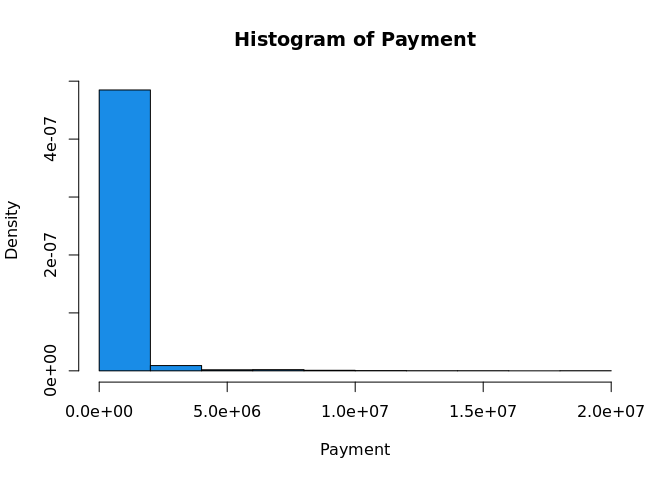
\includegraphics{README_files/figure-latex/unnamed-chunk-4-1.pdf}
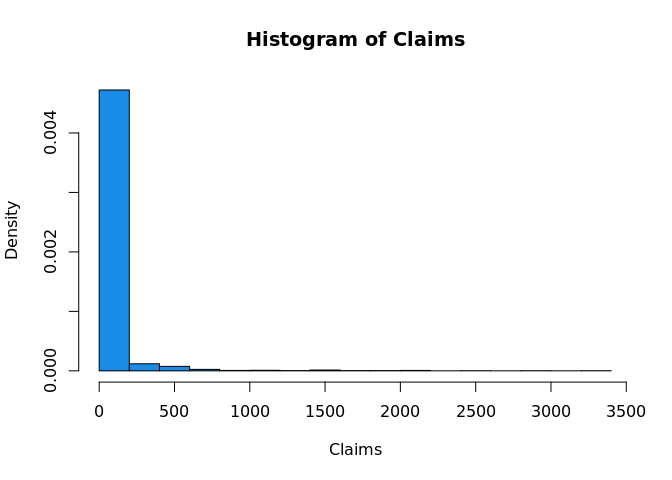
\includegraphics{README_files/figure-latex/unnamed-chunk-4-2.pdf}
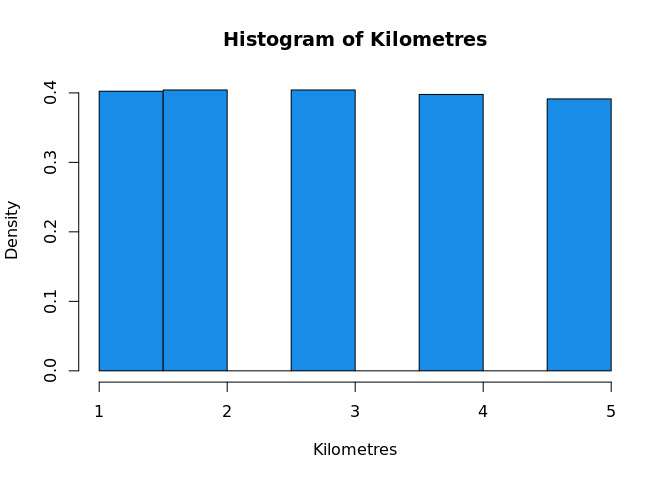
\includegraphics{README_files/figure-latex/unnamed-chunk-4-3.pdf}
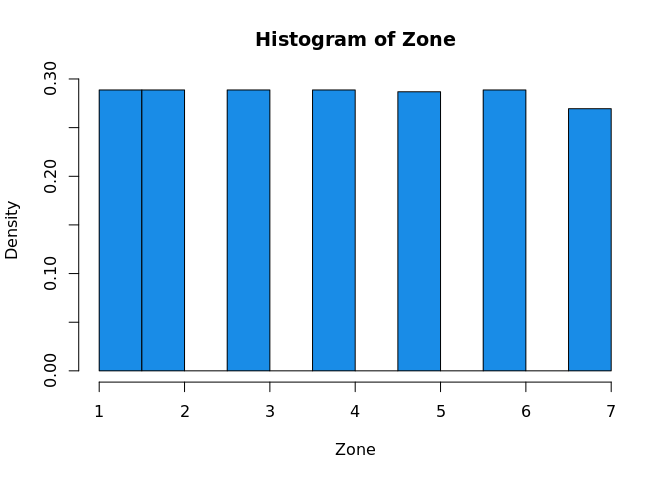
\includegraphics{README_files/figure-latex/unnamed-chunk-4-4.pdf}
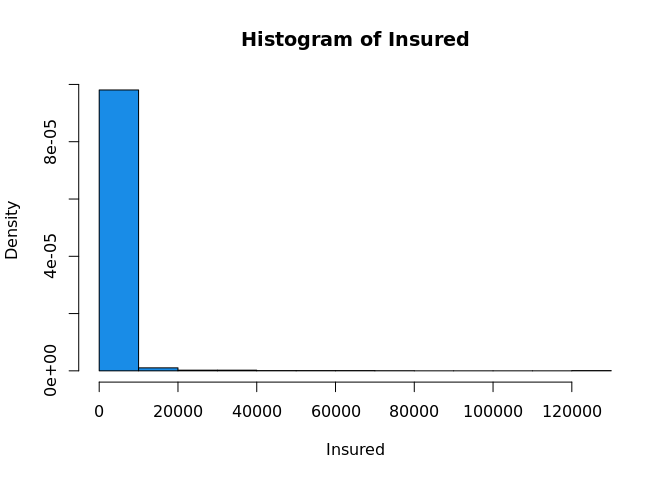
\includegraphics{README_files/figure-latex/unnamed-chunk-4-5.pdf}
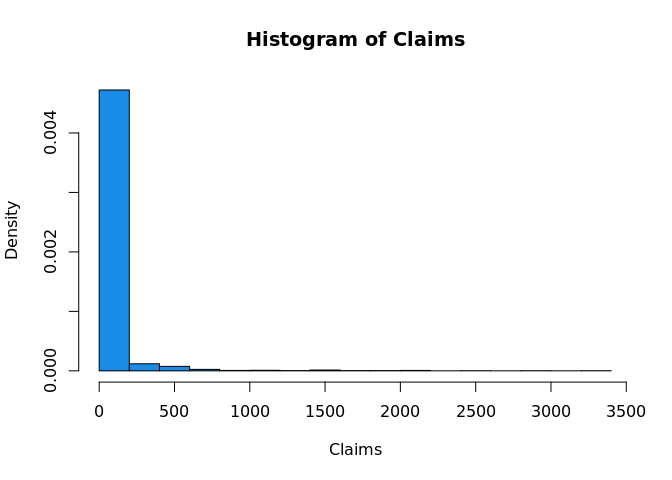
\includegraphics{README_files/figure-latex/unnamed-chunk-4-6.pdf}
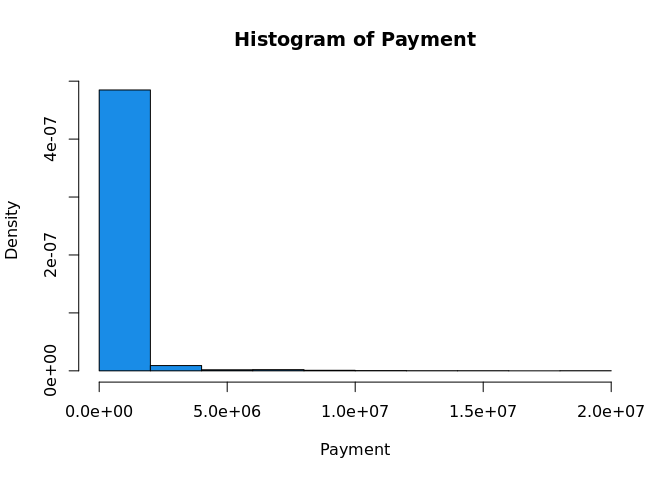
\includegraphics{README_files/figure-latex/unnamed-chunk-4-7.pdf}

\begin{verbatim}


\end{verbatim}

\end{document}
